%%%%%%%%%%%%%%%%%%%%%%%%%%%%%%%%%%%%%%%%%%%%%%%%%%%%%%%%%%%%%%%%%%%%%%%%

%%% LaTeX Template for AAMAS-2027 (based on sigconf.tex)
%%% Prepared by the AAMAS-2027 Publication Chairs based on the version from AAMAS-2026. 

%%%%%%%%%%%%%%%%%%%%%%%%%%%%%%%%%%%%%%%%%%%%%%%%%%%%%%%%%%%%%%%%%%%%%%%%

%%% Start your document with the \documentclass command.


%%% == IMPORTANT ==
%%% Use the first variant below to anonymize your submission (no author information shown).
%%% Use the second variant below for the final paper (including author information).
%%% For further information on anonymity and double-blind reviewing, 
%%% please consult the call for paper information
%%% https://warwick.ac.uk/fac/sci/dcs/aamas2027/calls/

%%%% For anonymized submission, use this
\documentclass[sigconf,anonymous]{aamas} 

%%%% For camera-ready, use this
%\documentclass[sigconf]{aamas} 


%%% Load required packages here (note that many are included already).

\usepackage{adjustbox}
\usepackage{subcaption} % for subfigure
\usepackage{balance} % for balancing columns on the final page

%%%%%%%%%%%%%%%%%%%%%%%%%%%%%%%%%%%%%%%%%%%%%%%%%%%%%%%%%%%%%%%%%%%%%%%%

%%% AAMAS-2027 copyright block (do not change!)

\makeatletter
\gdef\@copyrightpermission{
  \begin{minipage}{0.2\columnwidth}
   \href{https://creativecommons.org/licenses/by/4.0/}{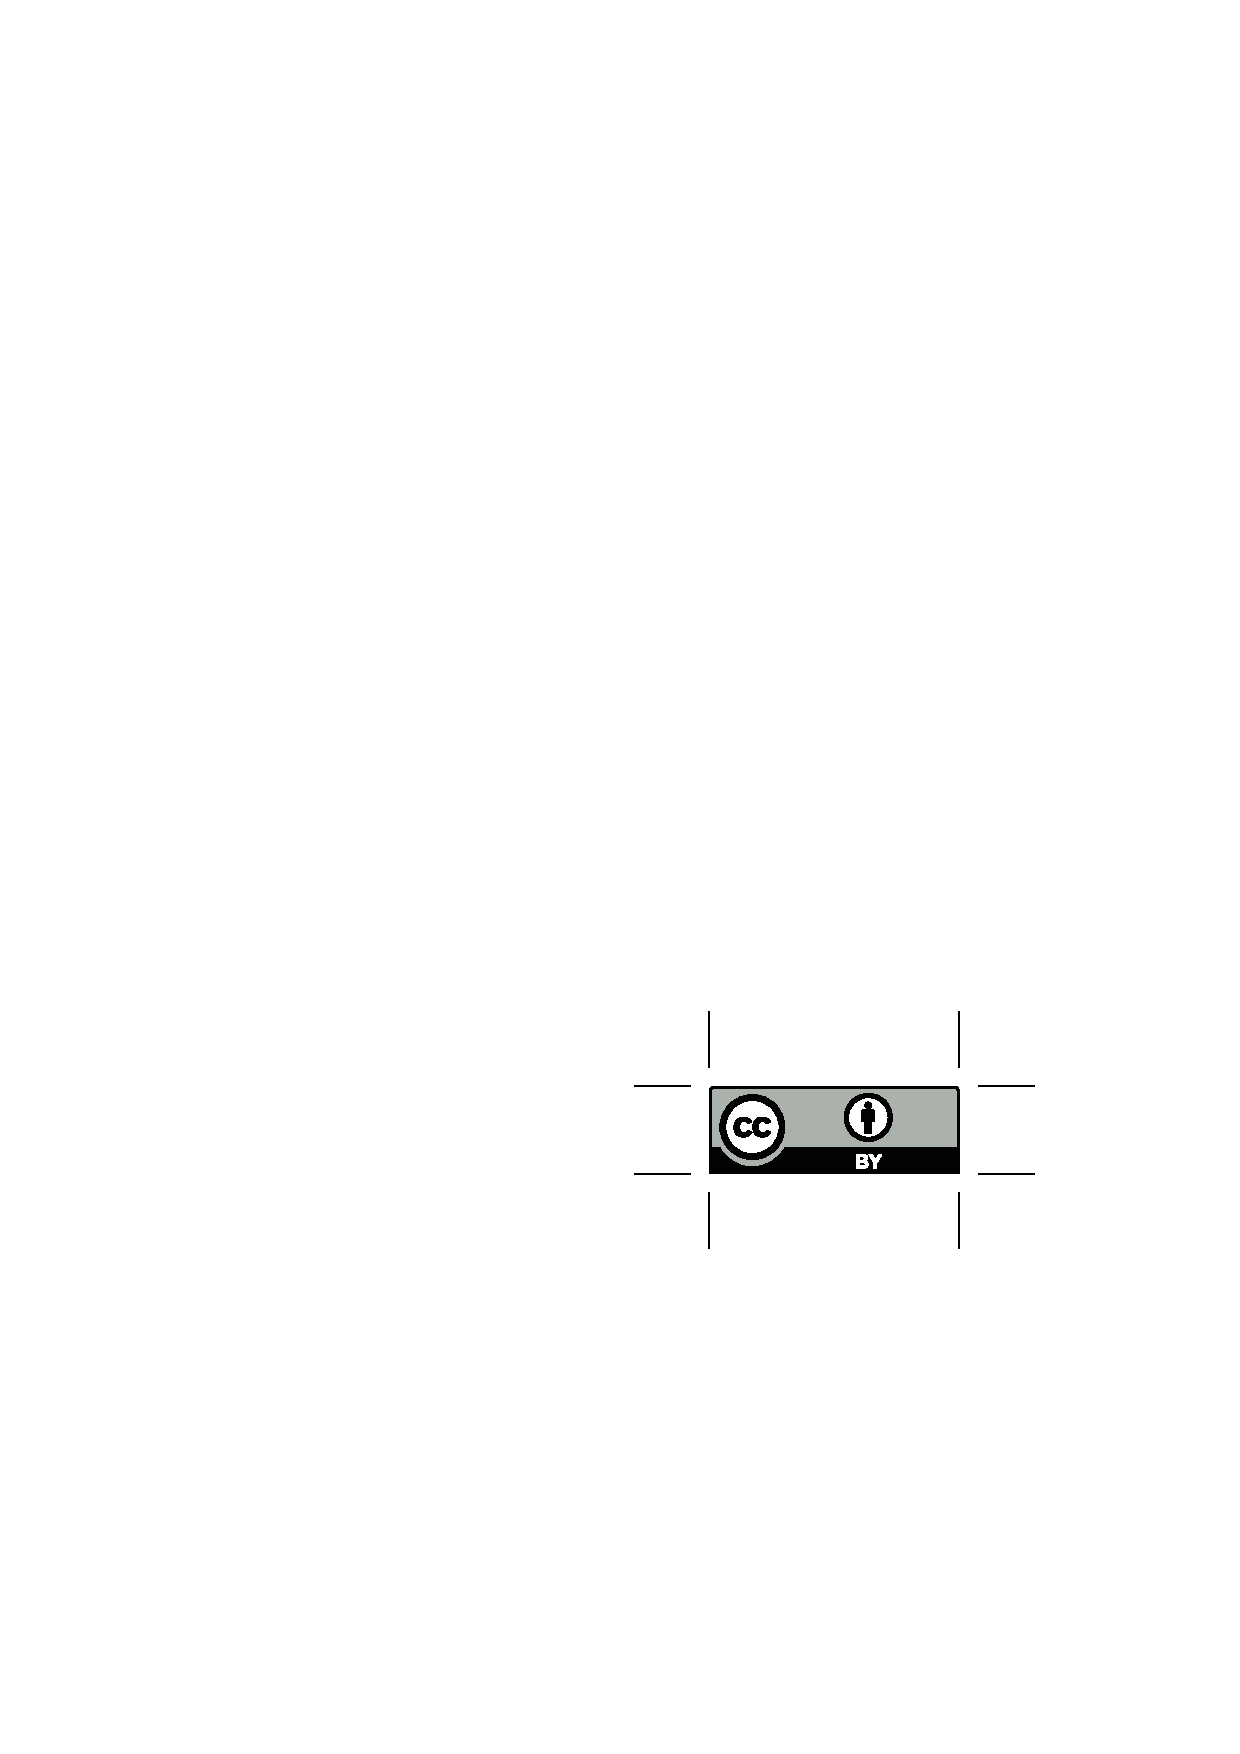
\includegraphics[width=0.90\textwidth]{by}}
  \end{minipage}\hfill
  \begin{minipage}{0.8\columnwidth}
   \href{https://creativecommons.org/licenses/by/4.0/}{This work is licensed under a Creative Commons Attribution International 4.0 License.}
  \end{minipage}
  \vspace{5pt}
}
\makeatother

\setcopyright{ifaamas}
\acmConference[AAMAS 2027]{Proc.\@ of the 26th International Conference
on Autonomous Agents and Multiagent Systems (AAMAS 2027)}{3--7 May 2027}{Hanoi, Vietnam}{M.~Baldoni, F.~Fang, W.~Yeoh, N.~Yorke-Smith (eds.)}
\copyrightyear{2027}
\acmYear{2027}
\acmDOI{}
%\acmPrice{}
\acmISBN{}

%%%%%%%%%%%%%%%%%%%%%%%%%%%%%%%%%%%%%%%%%%%%%%%%%%%%%%%%%%%%%%%%%%%%%%%%

%%% == IMPORTANT ==
%%% Use this command to specify your OpenReview submission number.
%%% In anonymous mode, it will be printed on the first page.

\acmSubmissionID{<<OpenReview submission id>>}

%%% Use this command to specify the track you want to submit your paper to.

\submissionType{Research Paper Track}
%\submissionType{AAAI Track}
%\submissionType{Demonstration Track}
%\submissionType{Blue Sky Ideas Track}
%\submissionType{JAAMAS Track}
%\submissionType{Doctoral Consortium}

%%% Use this command to specify the title of your paper.

\title[GENESIS: Stochastic Inference in MCTS for Automatic Heuristic Design]{Generative Exploration via Stochastic Inference in Monte Carlo Tree Search for Automatic Heuristic Design}

%%% Provide names, affiliations, and email addresses for all authors.

\author{Arthur Pendragon}
\affiliation{
  \institution{Camelot Castle}
  \city{Camelot}
  \country{United Kingdom}}
\email{king.arthur@camelot.uk}

\author{Nimue}
\affiliation{
  \institution{The Lady's Lake}
  \city{Avalon}
  \country{United Kingdom}}
\email{lady.of.the.lake@avalon.uk}

%%% Use this environment to specify a short abstract for your paper.

\begin{abstract}
Designing effective algorithmic components for NP-hard combinatorial optimization problems (COPs) remains a fundamental challenge, as traditional solvers predominantly rely on hand-crafted heuristics. While recent work uses large language models (LLMs) for automatic heuristic design (AHD), the resulting performance signals are highly noisy, as LLM-generated heuristics behave like samples from a high-variance stochastic process. Current approaches further reinforce this uncertainty by over-exploiting top-performing but fragile candidates. We propose GENeration Exploration via Stochastic Inference Monte Carlo Tree Search (GENESIS), an uncertainty-aware Monte Carlo Tree Search framework that models performance noise via Bayesian belief updating and integrates error-driven reflective reasoning. By explicitly modeling evaluation noise instead of averaging it away, GENESIS avoids over-committing to fragile candidates and surfaces robust ones from the same noisy LLM generator. Experiments on COP benchmarks show that GENESIS outperforms state-of-the-art LLM-AHD baselines in most problem instances under both ACO and construction framework settings. By transforming noisy trial-and-error into a structured search process, GENESIS offers a practical step toward fully automated algorithm design that requires less manual tuning and expert effort.
\end{abstract}

%%% Use this command to specify a few keywords describing your work.
%%% Keywords should be separated by commas.

\keywords{Automatic Heuristic Design, Large Language Models, Monte Carlo Tree Search, Thompson Sampling, Combinatorial Optimization}

%%%%%%%%%%%%%%%%%%%%%%%%%%%%%%%%%%%%%%%%%%%%%%%%%%%%%%%%%%%%%%%%%%%%%%%%

%%% Include any author-defined commands here.
         
\newcommand{\BibTeX}{\rm B\kern-.05em{\sc i\kern-.025em b}\kern-.08em\TeX}

%%%%%%%%%%%%%%%%%%%%%%%%%%%%%%%%%%%%%%%%%%%%%%%%%%%%%%%%%%%%%%%%%%%%%%%%

\begin{document}

%%% The following commands remove the headers in your paper. For final 
%%% papers, these will be inserted during the pagination process.

%\pagestyle{fancy}
%\fancyhead{}

%%% The next command prints the information defined in the preamble.

\maketitle

\section{Introduction}

Combinatorial optimization problems (COPs), such as vehicle routing, scheduling, and coverage planning, are NP-hard and arise across logistics, manufacturing, and robotics \cite{garey1979computers,Laporte2009VRP,Pinedo2016Scheduling,Tan2021CPP}. Due to their computational intractability, high-quality heuristics are essential for solving large-scale instances efficiently, yet designing such heuristics typically requires substantial domain expertise and manual tuning. This challenge has motivated hyper-heuristics (HH), also known as automatic heuristic design (AHD), which search over the space of heuristics rather than directly over the space of solutions \cite{Burke2010HH,Burke2013HH}. Earlier heuristic-generation approaches, often based on genetic programming, automatically composed heuristics from predefined building blocks \cite{langdon2002foundations,Epitropakis2025HH}. More recently, large language models (LLMs) have opened a new direction for AHD by enabling heuristic synthesis directly from natural-language descriptions. This LLM-based paradigm expands the search space beyond manually specified operators and has been explored together with evolutionary search and tree-search methods, yielding competitive performance with limited human intervention \cite{ye2024reevo,fei2024eoh,zheng2025montecarlo}.

\begin{figure}[!t]
    \centering
    \begin{subfigure}[b]{0.48\linewidth}
        \centering
        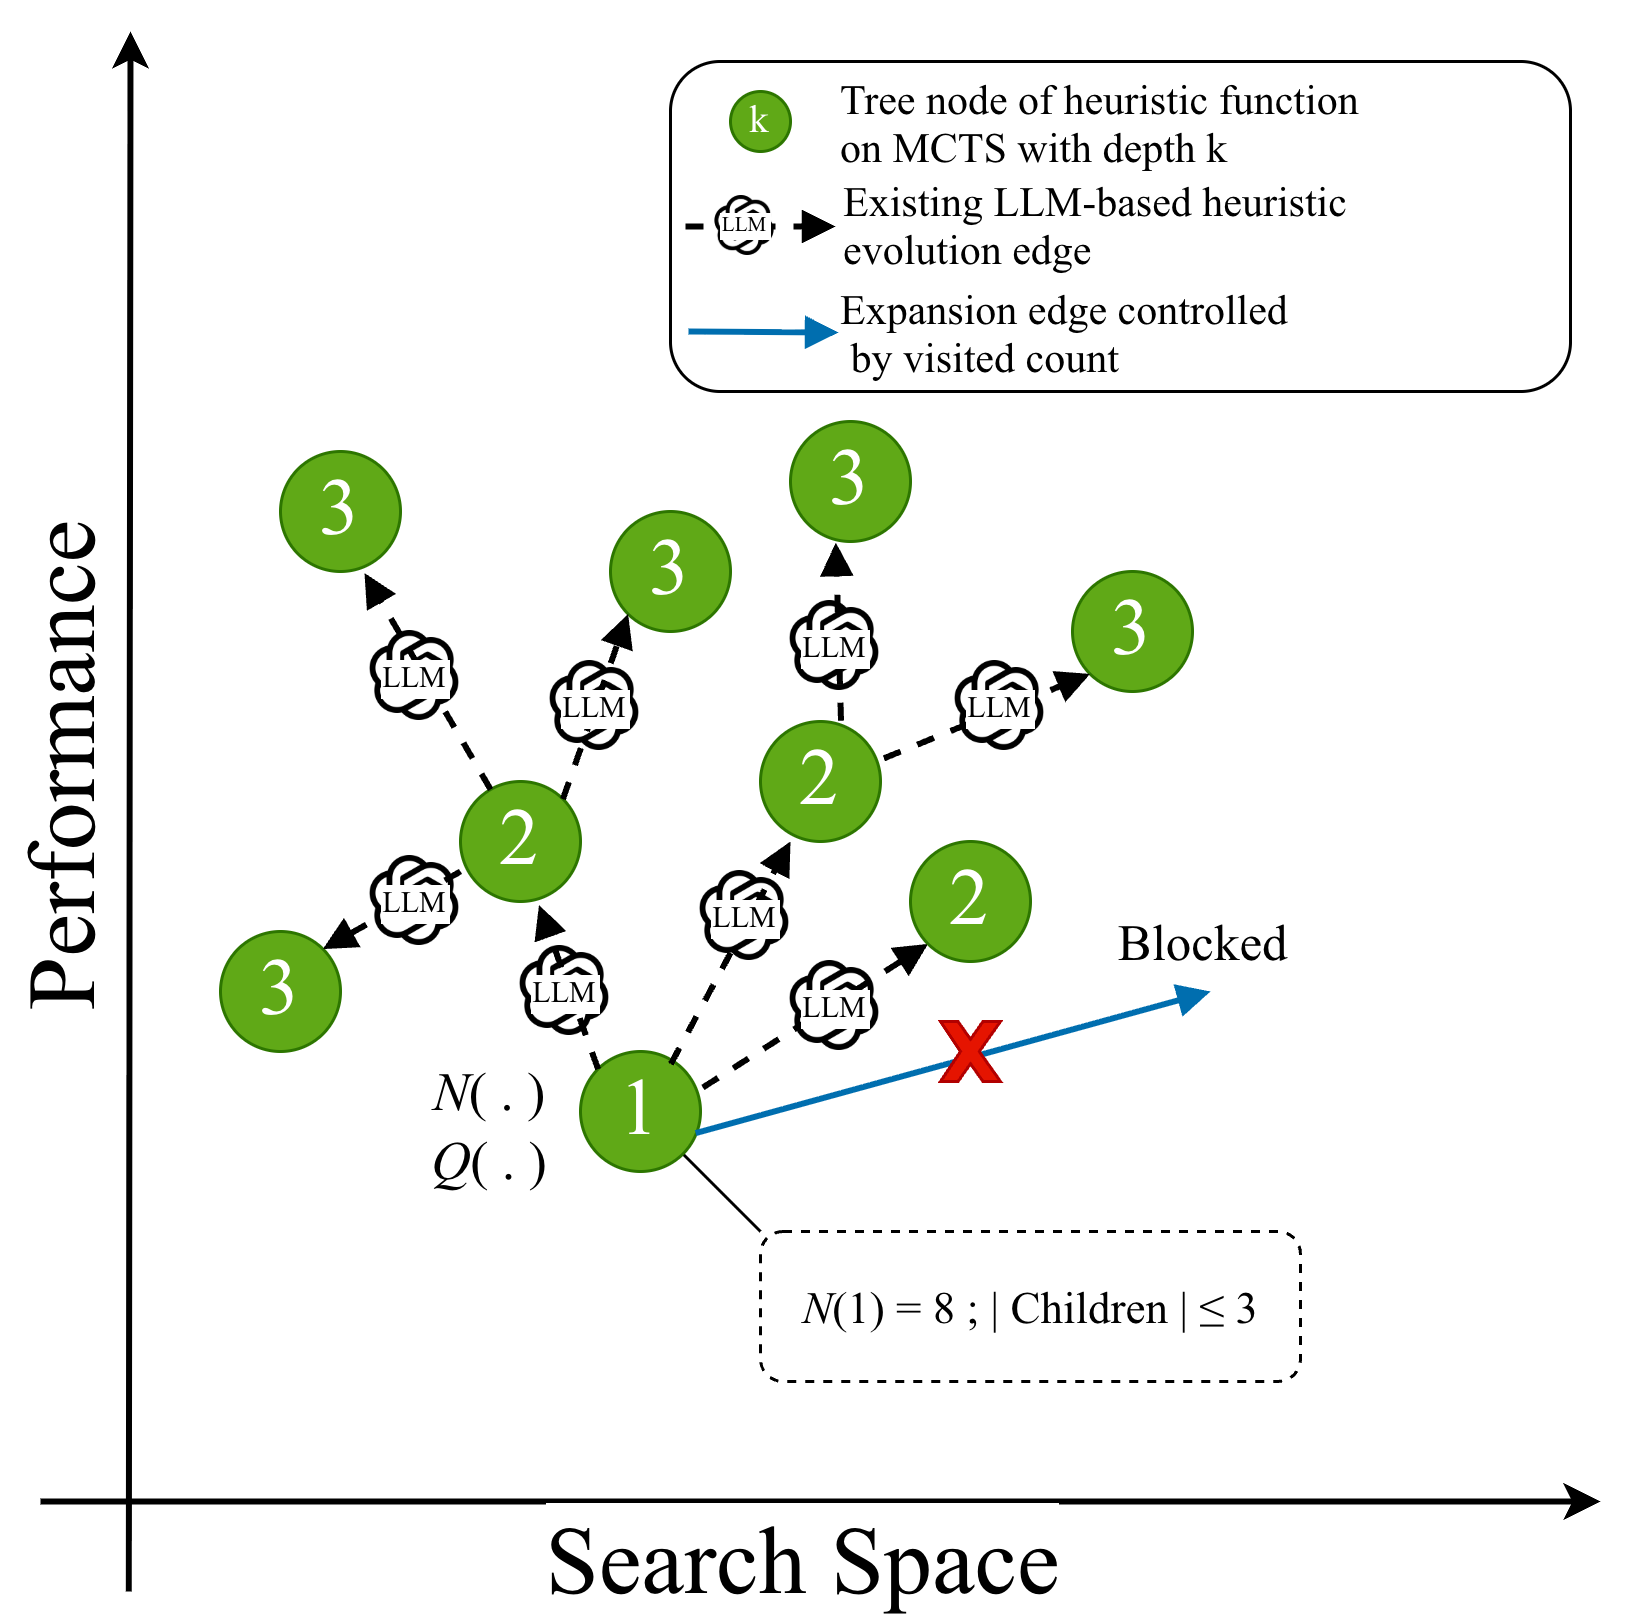
\includegraphics[width=\linewidth]{finMCTS.drawio.png}
        \caption{Progressive Widening}
        \label{fig:population_baseline}
    \end{subfigure}\hfill
    \begin{subfigure}[b]{0.48\linewidth}
        \centering
        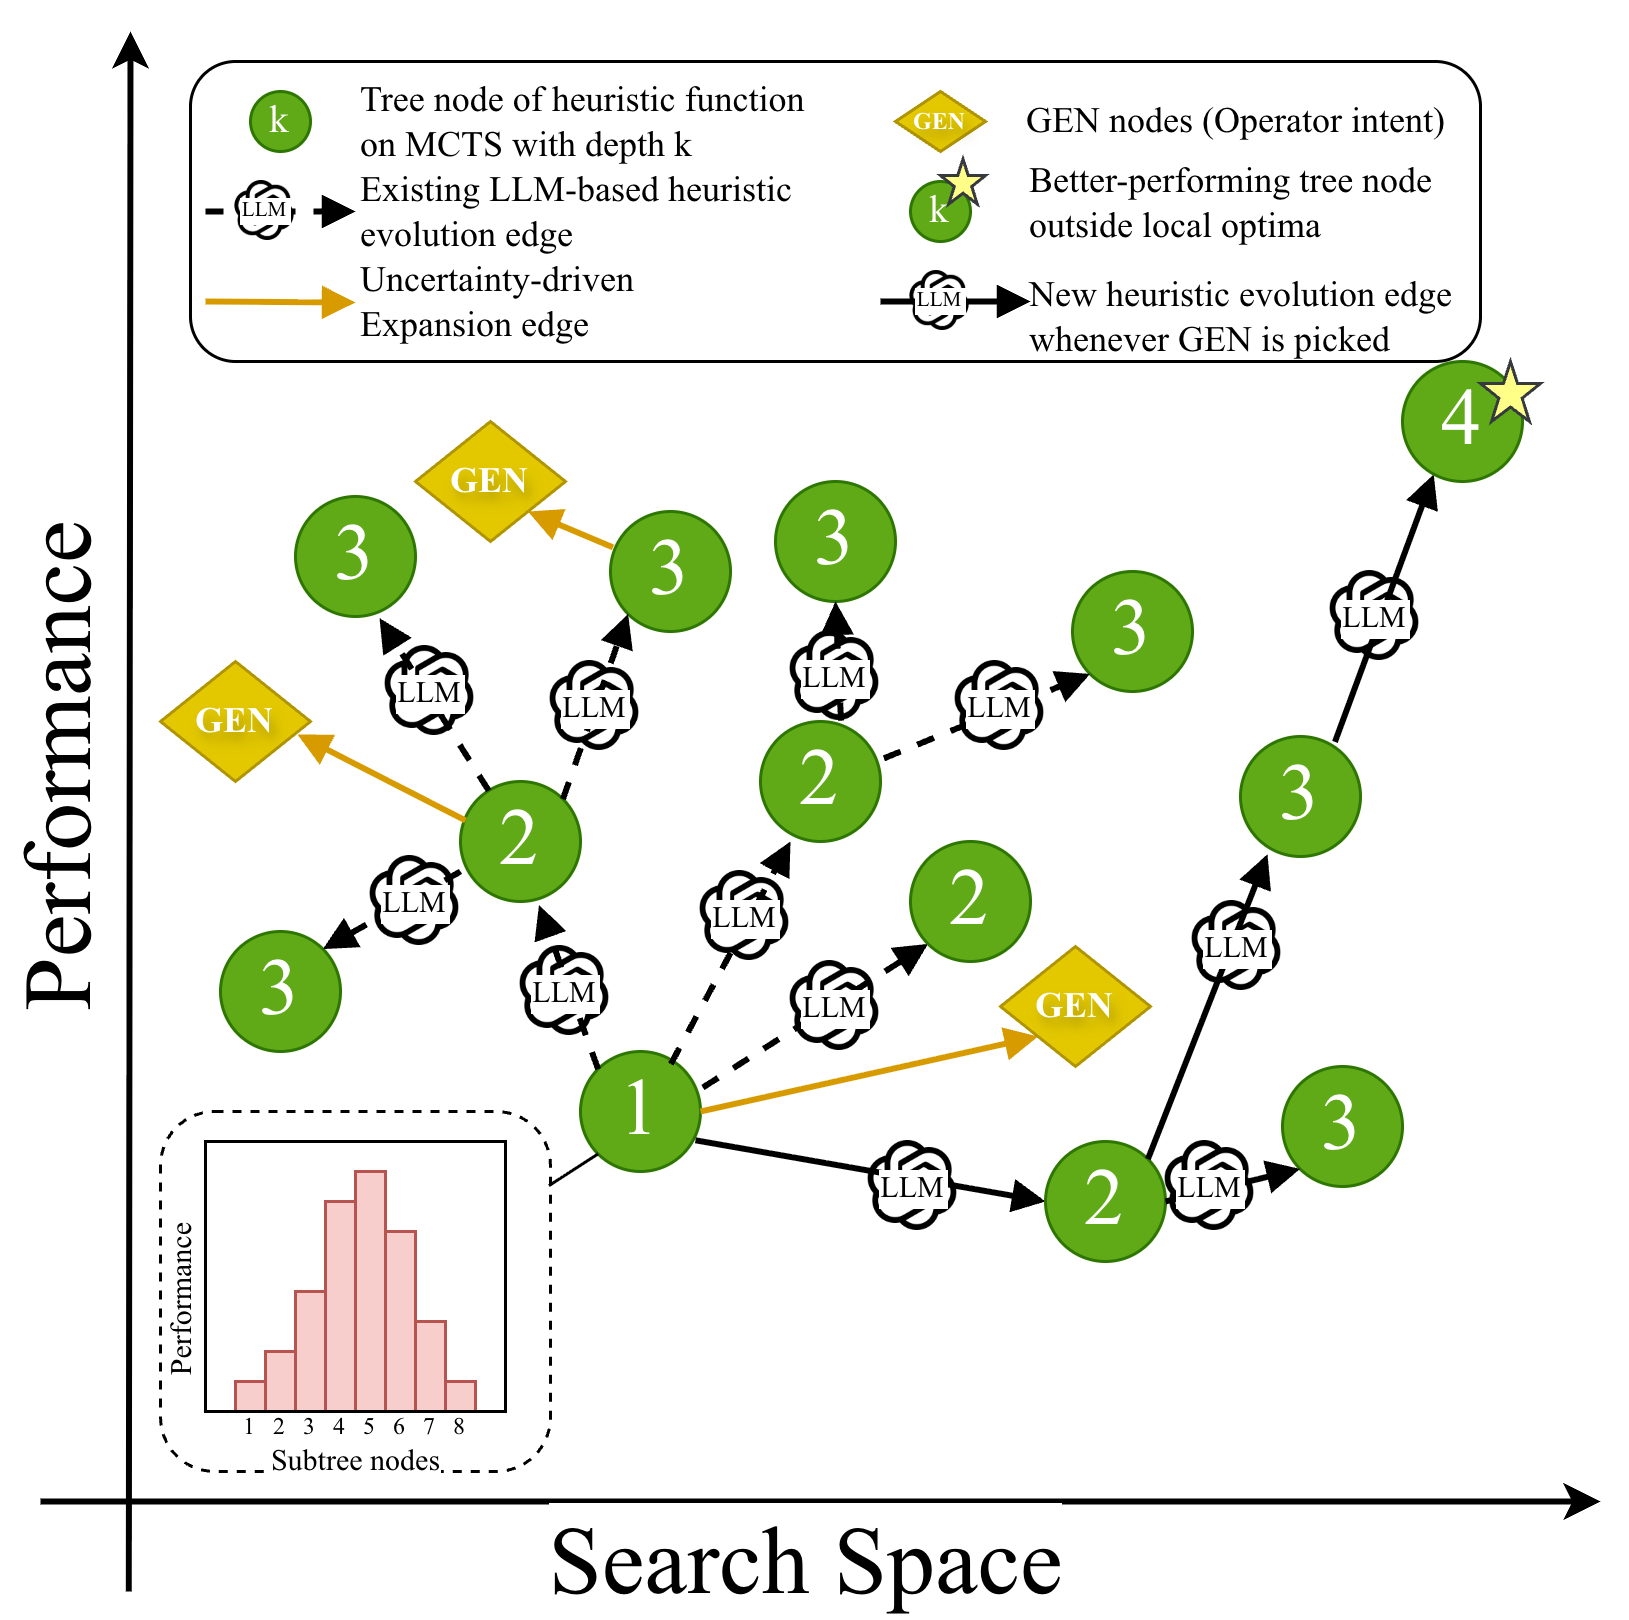
\includegraphics[width=\linewidth]{finMCTS Diagram.png}
        \caption{Adaptive Branching (Ours)}
        \label{fig:mcts_ours}
    \end{subfigure}
    \caption{Conceptual comparison between (a) Progressive Widening and (b) Adaptive Branching in GENESIS. Progressive Widening limits tree expansion using a visit-count-based quota, resulting in uniform and blind branching. In contrast, GENESIS introduces GEN nodes representing operator intents and performs uncertainty-aware branching via Hierarchical Thompson Sampling, enabling targeted and adaptive expansion toward promising regions.}
    \label{fig:comparison_strategies}
\end{figure}

Despite this promise, LLM-based AHD still faces fundamental limitations. LLM-generated heuristics are inherently stochastic and often highly sensitive to small prompt or semantic variations, so two generations from the same instruction can produce functionally different code with substantially different performance~\cite{Ouyang_2025}. As a result, heuristic evaluation in this setting is noisy rather than deterministic. Existing methods often respond to this noise by aggressively favoring currently best-performing candidates, which can lead to over-exploitation of fragile heuristics and premature rejection of more robust structures. Therefore, the key challenge in LLM-based AHD is not only how to generate new heuristics, but also how to search under uncertainty when the underlying generator itself is unstable.

To address these limitations, we introduce GENESIS, which reformulates tree search for language hyper-heuristics by modeling node values as random variables, enabling Thompson sampling exploration, and incorporating error-driven reflection inspired by human thinking. We conduct extensive experiments across multiple COP benchmarks and heuristic design settings, and the results show that our framework outperforms strong LLM-based AHD baselines in most settings, highlighting the value of uncertainty-aware search and reflective refinement. Our contributions can be summarized as follows:
\begin{itemize}
    \item We introduce a Bayesian Monte Carlo Tree Search (MCTS) framework that models node values as random variables with Normal--Inverse--Gamma priors and posteriors. By maintaining both global hyper-priors and local node posteriors, GENESIS explicitly captures evaluation uncertainty and reduces premature convergence to fragile heuristics.
    \item We propose a hierarchical Thompson sampling strategy for exploration-operator selection. By sampling from posterior beliefs at multiple levels of the search tree, GENESIS adaptively balances exploration and exploitation according to both uncertainty and observed performance.
    \item We introduce an error-driven reflection pipeline that simulates expert reasoning to refine heuristics during search through six sequential stages. This pipeline analyzes latent algorithmic weaknesses and counterfactual failures before generating revised code, thereby improving the robustness and generalizability of the discovered heuristics.
\end{itemize}
% noi them ve experiment


\section{Related Work}

\subsection{Language Hyper-Heuristic}


Recent approaches in automatic heuristic design leverage LLMs to generate, refine, or select heuristics from natural language prompts or high-level problem specifications. Methods such as FunSearch \cite{FunSearch2023}, AEL \cite{liu2023algorithmevolutionusinglarge}, EoH \cite{fei2024eoh}, ReEvo \cite{ye2024reevo}, HSEvo \cite{dat2025hsevo}, MCTS-AHD \cite{zheng2025montecarlo} and PoH \cite{wang2025planningheuristicsstrategicplanning} combine evolutionary search or tree search with LLM-generated heuristics. By iteratively generating, executing, and refining programs, these language-driven hyper-heuristics can discover high-quality, adaptable heuristics with minimal domain knowledge. 

\subsection{Distributional Monte Carlo Tree Search}

Distributional Monte Carlo Tree Search (MCTS) extends standard MCTS by modeling the full distribution of possible returns instead of only the expected value. This is particularly important in decision making under stochastic environment, where a single policy execution may have widely varying outcomes \cite{hayes2021riskawaremultiobjectivedecision, dam2023montecarlotreesearchuncertainty, anonymous2025distributional}. By maintaining a posterior over the utility of different returns, Distributional MCTS enables agents to make decisions that account for both risk and multiple objectives. Recent work has proposed a novel inference-time framework for LLMs that generalizes repeated sampling through principled multi-turn exploration and exploitation within tree search~\cite{inoue2025widerdeeperscalingllm}.


\section{Preliminaries}

\subsection{Problem Definition}

\begin{definition}[Language Hyper-Heuristic (LHH)]
Let $S$ denote the space of problem instances of a combinatorial optimization problem (COP), and let $H$ denote the space of heuristics for solving instances in $S$.  
Let $f: H \times S \to \mathbb{R}$ be a \emph{solver evaluation function} or an \emph{objective function}.

The \emph{meta-objective} $F: H \to \mathbb{R}$ is defined as the average performance of a heuristic $h$ over a dataset $\mathcal{I} \subseteq S$ of problem instances:
\[
F(h) = \frac{1}{|\mathcal{I}|} \sum_{i \in \mathcal{I}} f(h, i).
\]

Heuristics in $H$ may belong to diverse algorithmic frameworks, and an optimal heuristic may be expressible in multiple ways. To simplify design, LHH methods focus on a \emph{key heuristic function} with well-specified inputs and outputs; for example, in a step-by-step construction framework for the TSP, the key function selects the next city to visit given a partial tour. An LHH generates heuristics $h \in H$ probabilistically using a Large Language Model (LLM), conditioned on a seed heuristic $s_0 \in H$ and a natural-language prompt $a$:
\[
h \sim \mathrm{LLM}(s_0, a).
\]
The optimal heuristic under this generative model is
\[
% h^* = \arg\min_{h \sim \mathrm{LLM}(a)} F(h).
h^* = \arg\min_{h} F(h).
\]
Unlike traditional hyper-heuristics, which operate over a fixed, handcrafted set of low-level heuristics, LHHs do not require a predefined heuristic space, thereby enabling exploration of an open-ended, linguistically grounded space of heuristics.
\end{definition}

\subsection{Bayes' Theorem}

% Bayesian inference updates beliefs via Bayes' rule:
% \[
% p(\theta\mid D)\propto p(D\mid\theta)p(\theta).
% \]

% For univariate Gaussian rewards $x\sim\mathcal{N}(\mu,\sigma^2)$ with unknown $(\mu,\sigma^2)$, the conjugate prior is
% \[
% (\mu,\sigma^2)\sim\mathrm{NIG}(\mu_0,\kappa_0,\alpha_0,\beta_0).
% \]

% Given data with mean $\bar{x}$ and sum of squares $S=\sum_{i}(x_i-\bar{x})^2$, the posterior remains NIG with
% \[
% \kappa_n=\kappa_0+n,\quad
% \mu_n=\frac{\kappa_0\mu_0+n\bar{x}}{\kappa_0+n},
% \]
% \[
% \alpha_n=\alpha_0+\tfrac{n}{2},\quad
% \beta_n=\beta_0+\tfrac12\!\left(S+\frac{\kappa_0 n}{\kappa_0+n}(\bar{x}-\mu_0)^2\right).
% \]

Bayesian inference updates beliefs via Bayes' rule:
\[
p(\theta\mid D)\propto p(D\mid\theta)p(\theta).
\]
For univariate Gaussian rewards $x\sim\mathcal{N}(\mu,\sigma^2)$ with unknown $(\mu,\sigma^2)$, the conjugate prior is the \emph{Normal--Inverse--Gamma} (NIG) distribution,
\[
(\mu,\sigma^2)\sim\mathrm{NIG}(\mu_0,\kappa_0,\alpha_0,\beta_0),
\]
which factorizes as $\mathcal{N}\!\bigl(\mu \mid \mu_0, \sigma^2/\kappa_0\bigr) \cdot \mathrm{Inv\text{-}Gamma}(\sigma^2 \mid \alpha_0, \beta_0)$.
Given data with mean $\bar{x}$ and sum of squares $S=\sum_{i}(x_i-\bar{x})^2$, the posterior remains NIG with
\[
\kappa_n=\kappa_0+n,\quad
\mu_n=\frac{\kappa_0\mu_0+n\bar{x}}{\kappa_0+n},
\]
\[
\alpha_n=\alpha_0+\tfrac{n}{2},\quad
\beta_n=\beta_0+\tfrac12\!\left(S+\frac{\kappa_0 n}{\kappa_0+n}(\bar{x}-\mu_0)^2\right).
\]

% \subsection{Thompson Sampling}

% Thompson Sampling (TS) is a Bayesian approach to sequential decision-making under uncertainty~\cite{russo2020tutorialthompsonsampling}.
% In the $K$-armed Gaussian bandit setting, each arm $i$ generates rewards
% $r_i \sim \mathcal{N}(\mu_i, \sigma_i^2)$ with unknown parameters.
% At each round $t$, the parameters $(\mu_i, \sigma_i^2)$ of each arm are sampled from their NIG posterior, and a latent reward $\theta_i \sim \mathcal{N}(\mu_i, \sigma_i^2)$ is drawn.
% The selected arm is
% \[
% m = \arg\min_{i \in \{1, \dots, K\}} \theta_i,
% \]
% and the action pulling arm $m$ is applied, yielding the observed reward $r_{m,t}$.
% The NIG posterior of the selected arm is then updated.
% This posterior sampling mechanism naturally balances exploration and exploitation.


% \subsection{Hierarchical Thompson Sampling}

% Hierarchical Thompson Sampling (HTS) extends standard Thompson Sampling by introducing a shared global latent distribution that governs the reward structure across arms. Each arm \(i\) maintains a local NIG posterior over its unknown mean and variance \((\mu_i, \sigma_i^2)\), while a global NIG posterior models population-level parameters \((\mu_g, \sigma_g^2)\). At each round \(t\), the algorithm first samples global hyperparameters \((\mu_g, \sigma_g^2)\) from the current global posterior. It then assigns to every arm \(i\) a reward sample drawn directly from the global predictive distribution:
% \[
% \theta_i \sim \mathcal{N}(\mu_g, \sigma_g^2).
% \]
% The selected action is the arm with the smallest sampled value:
% \[
% m = \arg\min_{i \in \{1, \dots, K\}} \theta_i,
% \]
% and the observed reward \(r_{m, t}\) is used to update the local NIG posterior for the chosen arm. Optionally, the global NIG posterior is updated using aggregated sufficient statistics from all arms. By anchoring exploration to a shared global belief, this formulation enables strong information pooling across arms while maintaining coherent uncertainty quantification, which enhances sample efficiency in structured bandit problems~\cite{hong2022deephierarchybandits,hong2022hierarchicalbayesianbandits}.




\section{GENESIS Framework}

\subsection{Overall Architecture}

% GENESIS is an uncertainty-aware tree search framework for automatic heuristic design that combines adaptive-branching Monte Carlo Tree Search with hierarchical Bayesian modeling.
% The framework explores an open-ended heuristic space by iteratively generating and evaluating heuristics using a fixed set of operators.

% The search process is organized as a dynamically growing tree.
% Each \emph{real node} corresponds to a concrete heuristic $h$ with an observed meta-objective value $y_h$.
% From every real node, a shared set of \emph{operator nodes} is instantiated, one for each operator in
% \[
% \mathcal{O} = \{o_1,\dots,o_K\}.
% \]
% Operator nodes represent transformation directions and do not correspond to directly evaluable solutions.

% To enable principled selection despite missing immediate rewards, each node $u$ (real or operator) is associated with a latent meta-objective variable
% \[
% r_u \sim \mathcal{N}(\mu_u, \sigma_u^2),
% \]
% which models the distribution of meta-objective values of real nodes in the subtree rooted at $u$.
% Uncertainty over $(\mu_u, \sigma_u^2)$ is modeled using NIG priors.

% Operator nodes aggregate evidence from all heuristics generated via the same operator and are coupled through a shared global hyper-prior, allowing statistical strength to be shared across the tree.
% Tree traversal and expansion are driven by TS: at each decision point, a latent value is sampled from each candidate node’s posterior, and the node with the minimum sample is selected.
% Selecting a real node continues traversal, while selecting an operator node triggers the generation of new heuristics, which are added as real nodes.
% Observed meta-objectives are propagated upward to update local and global posteriors.

% GENESIS further incorporates an \emph{Assumption-Guided Reflective Expansion} (AGRE) module, which analyzes high-performing heuristics to surface fragile assumptions and guide subsequent heuristic generation toward more robust designs.

GENESIS is an uncertainty-aware tree search framework for automatic heuristic design that combines adaptive Monte Carlo Tree Search with hierarchical Bayesian modeling (Figure~\ref{fig:comparison_strategies}). It explores an open-ended heuristic space by iteratively generating and evaluating heuristics using a fixed set of operators.

The search is organized as a dynamically growing tree with two types of nodes: \emph{real nodes}, representing concrete heuristics with observed meta-objective values, and \emph{operator nodes}, representing abstract transformation directions shared across the tree. Operator nodes do not correspond to directly evaluable solutions but aggregate evidence from heuristics generated by the same operator.

Each node is associated with a latent performance variable modeling the distribution of meta-objective values in its subtree, with uncertainty captured via Bayesian priors. Tree traversal is guided by Thompson Sampling, enabling principled selection under uncertainty: selecting a real node continues traversal, while selecting an operator node triggers heuristic generation and expansion. Observed evaluations are propagated upward to update both local and shared uncertainty estimates.

GENESIS further incorporates an \emph{Assumption-Guided Reflective Expansion (AGRE)} module, which analyzes high-performing heuristics to identify fragile assumptions and guide subsequent generation toward more robust designs.

\subsection{Detailed Algorithm}

\subsubsection{Problem Setup}

The search process is initialized with an empty root node \(s_0\). An initial set of \(N_0\) heuristics is generated and added as real child nodes of \(s_0\), forming the first level of the search tree. Each node $s$ in the search tree maintains two types of children:
(i) a set of \emph{real child nodes} $\mathcal{R}(s)$, each representing a concrete heuristic obtained by applying an operator, and
(ii) a set of \emph{operator nodes} $\mathcal{G}(s)$, with one operator node associated with each operator in the operator set $\mathcal{O} = \{o_1,\dots,o_K\}$. Operator nodes represent abstract transformation actions and do not correspond to directly evaluable heuristics.

For every node \(s\) in the search tree (real or operator or root), the algorithm maintains a local Bayesian posterior over a latent meta-objective parameter \(\theta_s\), modeled using a NIG distribution:
\begin{equation}
(\mu_s, \sigma_s^2) \sim \mathrm{NIG}(\mu_0, \kappa_0, \nu_0, \tau_0^2).
\end{equation}
Evaluation outcomes are assumed to follow
\begin{equation}
\theta_s \mid \mu_s, \sigma_s^2 \sim \mathcal{N}(\mu_s, \sigma_s^2).
\end{equation}
The resulting posterior compactly summarizes all evaluation evidence collected for the corresponding heuristic or operator node. To enable statistical sharing across operator nodes, a global hyper-prior $\text{NIG}(\mu_{global}, \kappa_{global}, \nu_{global}, \tau_{global}^2)$ is defined and shared across all operator nodes in the tree. This hyper-prior governs the prior distribution of operator-level performance and is updated incrementally as new heuristics are generated and evaluated during the search.

\subsubsection{Selection}

% The search process is initialized with a virtual root node \(s_0\). A set of initial heuristics with $N_0$ node is generated and added as real child nodes of \(s_0\). Starting from $s_0$, the algorithm performs TS and HTS to guide tree traversal.

% A global latent performance parameter $(\mu_g, \sigma_g^2)$ is first sampled from the shared NIG hyper-posterior. This global sample is shared across all operator nodes, since they are all rely on a common LLM to expand the tree. 


% For each real child node $r$, a local posterior sample $(\mu_r, \sigma_r^2)$ is drawn from its NIG posterior.
% HTS then combines global and local information via precision-weighted updating:
% \[
% \lambda_r
% = \frac{\kappa_r / \sigma_r^2}{\kappa_r / \sigma_r^2 + \kappa_g / \sigma_g^2},
% \]
% \[
% \mu_r^{\star}
% = \lambda_r \mu_r + (1-\lambda_r)\mu_g,
% \]
% \[
% (\sigma_r^{2})^{\star}
% = \left( \frac{\kappa_r}{\sigma_r^2} + \frac{\kappa_g}{\sigma_g^2} \right)^{-1},
% \]
% \[
% \theta_r
% \sim \mathcal{N}\!\left(\mu_r^{\star}, (\sigma_r^{2})^{\star}\right).
% \]

% This update jointly shrinks both the mean and variance toward the operator-level belief, with the degree of shrinkage controlled by relative posterior precision.

% In contrast, real nodes are treated as conditionally independent and do not share information with one another.Although they come from the same parent, each real node represents a different heuristic instance. By keeping their uncertainties separate, we avoid over-favoring unreliable heuristics during selection.

% The algorithm selects the node with the most favorable sampled value.
% If a real node is selected, selection continues recursively; otherwise, selecting an operator node terminates selection and triggers expansion.

The search process is initialized with a virtual root node \( s_0 \). A set of initial heuristics with \( N_0 \) nodes is generated and added as real child nodes of \( s_0 \). Starting from \( s_0 \), the algorithm performs Thompson Sampling (TS) and Hierarchical Thompson Sampling (HTS) to guide tree traversal. At each state \( s \), a global latent performance parameter \( (\mu_0, \sigma_0^2) \) is first sampled from a shared global NIG hyper-posterior. This global sample is shared across all operator nodes \( g \in \mathcal{G}(s) \), since they all rely on a common LLM to expand the tree. For each operator child node \( g \in \mathcal{G}(s) \), a local posterior sample \( (\mu_g, \sigma_g^2) \) is drawn from its NIG posterior. HTS then combines global and operator-level information via precision-weighted updating:
\[
\lambda_g
= \frac{\kappa_g / \sigma_g^2}{\kappa_g / \sigma_g^2 + \kappa_0 / \sigma_0^2},
\]
\[
\mu_g^{\text{comb}}
= \lambda_g \mu_g + (1-\lambda_g)\mu_0,
\]
\[
\sigma_g^{2,\text{comb}}
= \left( \frac{\kappa_g}{\sigma_g^2} + \frac{\kappa_0}{\sigma_0^2} \right)^{-1},
\]
\[
\theta_g
\sim \mathcal{N}\!\left(\mu_g^{\text{comb}}, \sigma_g^{2,\text{comb}}\right).
\]
This hierarchical update jointly shrinks both the mean and variance of operator nodes toward the global belief, with the degree of shrinkage controlled by their relative posterior precision. In contrast, real child nodes \( r \in \mathcal{R}(s) \) are treated as conditionally independent and are sampled solely from their local NIG posteriors:
\[
(\mu_r^{\text{loc}}, \sigma_r^{2,\text{loc}}) \sim \text{NIG}_r,
\qquad
\theta_r \sim \mathcal{N}(\mu_r^{\text{loc}}, \sigma_r^{2,\text{loc}}).
\]
Although they may originate from the same operator, each real node represents a distinct heuristic instance. By maintaining separate uncertainty estimates, the algorithm avoids over-favoring unreliable heuristics during selection. The algorithm selects the node with the most favorable sampled value,
\[
s^* \;\gets\; \arg\min_{x \in \mathcal{G}(s) \cup \mathcal{R}(s)} \theta_x .
\]
If a real node is selected, the selection process continues recursively from that node; otherwise, selecting an operator node terminates selection and triggers expansion.



\subsubsection{Expansion}

We design several LLM-based operators to generate new heuristics from existing ones. After a node is selected for expansion, the operator corresponding to the chosen operator node is applied to generate $N$ new child heuristics, which are added to the search tree as real nodes.

\textbf{E1 (Diversity-driven generation).}
Given multiple existing heuristics and their meta-objective values, the LLM generates a new heuristic that is structurally and algorithmically as different as possible from all provided ones, aiming to explore novel designs with lower meta-objective value.

\textbf{E2 (Idea-guided recombination).}
Given several heuristics, the LLM first identifies common effective ideas from a reference heuristic and then designs a new heuristic inspired by these ideas while modifying the structure of another selected heuristic, with the goal of outperforming both parents.

\textbf{M1 (Structural modification).}
Given a single heuristic, the LLM produces a modified version by introducing new mechanisms, equations, or program components, while preserving the core idea of the original algorithm.

\textbf{M2 (Parameter variation).}
Given a single heuristic, the LLM generates a new variant by identifying key algorithmic parameters and altering their values or configurations, without changing the overall algorithmic structure.

\textbf{S1 (Synthesis).}
Given multiple heuristics, the LLM extracts useful ideas from all of them and synthesizes a new heuristic that combines these insights to achieve better performance than any individual parent.

\textbf{NS (Novelty Search).}
Given a heuristic, the LLM explicitly analyzes its weaknesses, inefficiencies, or limitations and constructs a new heuristic that exploits these vulnerabilities to counter or outperform the original approach.

\subsubsection{Backpropagation}

After expansion and evaluation, the observed meta-objective values of the newly generated children are propagated backward along the path $\mathcal{P}$ from the root $s_0$. For each node $u \in \mathcal{P}$, the local NIG posterior is updated using the meta-objective values obtained from these newly generated nodes, thereby refining the node-specific uncertainty estimates.

In addition, whenever a node $u$ corresponds to an operator node, its observations are also used to update the global NIG hyper-posterior.
This global update aggregates evidence across all operator nodes generated by the same LLM-based transformation process, enabling principled statistical sharing while maintaining a conservative uncertainty estimate.


\subsubsection{Assumption-Guided Reflective Expansion}

Recent studies suggest that LLMs exhibit dual-process reasoning, combining fast intuitive responses with slower deliberative processes \cite{Hagendorff_2023,chung2025thinkerlearningthinkfast}. While prior work primarily applies this paradigm to output-level refinement in question–answering, human experts also critically examine and revise the \emph{assumptions} underlying solutions and algorithms.

Motivated by this observation, we propose \textit{Assumption-Guided Reflective Expansion (AGRE)}, a structured pipeline that extends fast–slow reasoning to assumption-level analysis. AGRE proceeds through six stages, each corresponding to a distinct cognitive function in human expert reasoning.

\textbf{Fast Intuitive Error Signaling.}
The LLM is prompted to generate brief, intuition-driven ``discomfort signals''
regarding the algorithm, highlighting brittle design choices, implicit
assumptions, or potential silent failure modes.
No proofs, fixes, or detailed explanations are allowed.
This stage corresponds to fast, intuitive anomaly detection (System~1) \cite{kahneman2011thinking}.

\textbf{Minimal Counterfactual Failure Construction.}
Conditioned on the detected error signals, the model constructs a single,
minimal, and realistic scenario in which the algorithm fails due to a broken
assumption.
The emphasis is on plausibility rather than extremity, following classical
theories of counterfactual reasoning in cognitive psychology
\cite{roese1997counterfactual}.
This step transforms vague intuition into a concrete failure hypothesis.

\textbf{Role-Based Reflective Conflict.}
The algorithm is examined through three explicitly separated roles:
(i) a \emph{Defender}, which justifies the original design under its intended assumptions;
(ii) an \emph{Attacker}, which argues that counterfactuals expose fundamental weaknesses; and
(iii) an \emph{Observer}, which synthesizes the remaining epistemic tension.
This structured internal debate is inspired by the argumentative theory of reasoning, which holds that robust judgments emerge from adversarial evaluation of competing explanations \cite{mercier2011why}. It is further supported by recent work on adversarial prompting and debate-based LLM reasoning, showing that explicit role opposition and self-critique improve factuality and error detection \cite{irving2018aisafetydebate,du2023improvingfactualityreasoninglanguage,madaan2023selfrefineiterativerefinementselffeedback}.


\textbf{Strategic Abstraction.}
The analysis is lifted from implementation details to a higher level of
abstraction, focusing on the algorithm's core strategy, trade-offs, and
assumption structure. This abstraction step prevents overfitting to surface-level artifacts and supports transferable insight across problem instances.

\textbf{Assumption Repair via Metacognitive Regulation.}
Rather than modifying the algorithm itself, AGRE refines or restricts only the
algorithm's assumptions or applicability conditions. This mirrors metacognitive regulation in human problem solving, where robustness
is improved by clarifying when a heuristic should or should not be trusted
\cite{flavell1979}. 

 \textbf{Assumption-Conditioned Refinement Guidance.}
Finally, the repaired assumptions are translated into concrete, implementable
guidance for improving robustness, stability, or generalization, while
preserving the original algorithmic intent.

After generating $N$ candidate child heuristics, the child with the lowest meta-objective value is selected for AGRE. The resulting heuristic is appended to the search tree, and its evaluation outcome is propagated backward along the path to the root.


\section{Experiments}

\begin{table*}[!tp]
\centering
\small
\caption{
Performance comparison on combinatorial optimization problems under the ACO framework.
Results report average objective values ($\pm$ standard deviation) over 3 runs; the evaluation dataset consists of 64 instances for each problem and instance size.
Lower is better ($\downarrow$) for TSP, CVRP, and BPP; higher is better ($\uparrow$) for MKP. Best results are in bold.
}
\label{tab:main_results}

\begin{tabular*}{\textwidth}{@{\extracolsep{\fill}}llccccc@{}}
\toprule
Problem & Size & EoH & ReEvo & HSEvo & MCTS-AHD & GENESIS \\
\midrule
TSP $\downarrow$ & 20   & 3.867 $\pm$ 0.002 & 3.878 $\pm$ 0.010 & 3.874 $\pm$ 0.011 & 3.878 $\pm$ 0.010 & \textbf{3.866 $\pm$ 0.003} \\
                 & 50   & 5.860 $\pm$ 0.013 & 5.862 $\pm$ 0.003 & 5.871 $\pm$ 0.022 & 5.862 $\pm$ 0.003 & \textbf{5.807 $\pm$ 0.076} \\
                 & 100  & 8.453 $\pm$ 0.028 & 8.442 $\pm$ 0.079 & 8.388 $\pm$ 0.029 & 8.442 $\pm$ 0.079 & \textbf{8.385 $\pm$ 0.133} \\
\midrule
CVRP $\downarrow$ & 20  & 4.919 $\pm$ 0.056 & 5.013 $\pm$ 0.185 & 4.931 $\pm$ 0.193 & 4.959 $\pm$ 0.079 & \textbf{4.842 $\pm$ 0.032} \\
                  & 50  & 9.588 $\pm$ 0.163 & 9.595 $\pm$ 0.311 & 9.629 $\pm$ 0.247 & 9.503 $\pm$ 0.063 & \textbf{9.004 $\pm$ 0.347} \\
                  & 100 & 17.039 $\pm$ 0.476 & 16.503 $\pm$ 0.992 & 16.868 $\pm$ 0.426 & 16.544 $\pm$ 0.170 & \textbf{15.827 $\pm$ 0.244} \\
\midrule
MKP $\uparrow$ & 100    & 16.850 $\pm$ 0.158 & 17.013 $\pm$ 0.034 & 16.945 $\pm$ 0.065 & \textbf{17.066 $\pm$ 0.017} & 17.048 $\pm$ 0.037 \\
               & 300    & 51.936 $\pm$ 0.768 & 53.556 $\pm$ 0.662 & 46.793 $\pm$ 8.028 & 53.222 $\pm$ 1.308 & \textbf{53.993 $\pm$ 0.191} \\
               & 500    & 124.067 $\pm$ 1.383 & 130.687 $\pm$ 1.771 & 128.331 $\pm$ 3.399 & 129.781 $\pm$ 1.099 & \textbf{131.044 $\pm$ 0.948} \\
\midrule
BPP $\downarrow$ & 120  & 49.531 $\pm$ 0.095 & 49.828 $\pm$ 0.053 & 49.661 $\pm$ 0.307 & 49.682 $\pm$ 0.180 & \textbf{49.453 $\pm$ 0.041} \\
                 & 500  & 205.115 $\pm$ 0.070 & 206.505 $\pm$ 0.503 & 205.474 $\pm$ 0.609 & 205.177 $\pm$ 0.095 & \textbf{204.865 $\pm$ 0.048} \\
                 & 1000 & 409.208 $\pm$ 0.079 & 412.182 $\pm$ 1.340 & 410.271 $\pm$ 1.220 & 408.984 $\pm$ 0.688 & \textbf{408.719 $\pm$ 0.016} \\
\bottomrule
\end{tabular*}
\end{table*}


\subsection{Experimental Setting}

%gop language model va setting
\paragraph{Language Model.}
All experiments are conducted using \texttt{codestral-2508}. This model is accessed via the official Mistral API using publicly available (free-tier) API keys. Despite the absence of paid or proprietary fine-tuning, Codestral demonstrates strong code generation and program synthesis capabilities.
\paragraph{Benchmark.}We compare GENESIS with other LHH baselines within an Ant Colony Optimization (ACO) framework. All methods share the same underlying ACO construction process and differ only in how heuristics or operators are generated and selected. The comparison spans four combinatorial optimization problems:
Traveling Salesman Problem (TSP), Multiple Knapsack Problem
(MKP), Capacitated Vehicle Routing Problem (CVRP), and Offline Bin Packing
Problem (Offline BPP). For TSP and KP, both offline heuristic generation and step-by-step solution construction settings are considered.
\paragraph{Setting.} All experiments are conducted on a single Intel Core i7-10850H CPU. For all problem instances, the maximum wall-clock time for heuristic
design is limited to $60$s. For ACO-based methods, the maximum number of function evaluations is set to $500$, while for step-by-step constructive methods, the evaluation budget is increased to $1{,}000$. The initial heuristic pool size is set to $N_0 = 5$.
During tree expansion, each operator node generates $N = 4$ new candidate heuristics. All methods share the same evaluation interface and objective functions. For each LLM-based AHD baseline, we perform three independent runs and
report the average performance, while selecting the best result among
the three runs for comparison.

\subsection{Results}

\paragraph{Ant Colony Optimization (ACO).}
Ant Colony Optimization (ACO) is a population-based metaheuristic inspired by the foraging behavior of ants, originally introduced as the Ant System \cite{dorigo1996ant} for solving combinatorial optimization problems. In ACO, artificial ants iteratively construct solutions by traversing a problem graph according to probabilistic transition rules that balance pheromone intensity and heuristic information. Pheromone trails are updated based on solution quality, reinforcing promising solution components over time. The Ant Colony System (ACS) further improves this framework through local pheromone updates and elitist reinforcement strategies \cite{dorigo1997ant}. Within this paradigm, the heuristic matrix plays a central role in guiding path selection by encoding problem-specific instance information. By parameterizing or generating this heuristic matrix, external models can directly influence the solution construction process, effectively transforming ACO into a general-purpose optimization framework. In this work, we leverage LLM-based automatic heuristic design (AHD) to generate heuristic functions, enabling ACO to be flexibly applied across a diverse set of combinatorial optimization problems. Table~\ref{tab:main_results} compares the performance of GENESIS with other baseline LHHs. The test dataset consists of 64 instances for every problem and instance size.



% Old version of the step-by-step paragraph with three separate tables;
% superseded by the merged Table~\ref{tab:constructive_merged} below.
\iffalse
\paragraph{Step-by-Step Construction Framework.}

We evaluate GENESIS and competing with other LHH frameworks under the \emph{step-by-step construction} setting, where a feasible solution is incrementally built by selecting and appending solution components based on the current partial state \cite{asani2023convexhull,bello2017neuralcombinatorialoptimizationreinforcement}. This framework is general and applies uniformly across routing, packing, and synthetic combinatorial construction problems.


For the Traveling Salesman Problem (TSP), solutions are constructed by iteratively selecting the next city until a complete tour is formed. Results are reported in Table~\ref{tab:tsp_constructive_transposed}.

\begin{table}[!htbp]
\centering
\scriptsize
\setlength{\tabcolsep}{3pt}

\caption{Average tour length over 3 runs for LHH frameworks on TSP constructive instances. Evaluation is performed on 64 instances per size with numbers of cities $\{20,50,100,200\}$. Lower values are better ($\downarrow$).}
\label{tab:tsp_constructive_transposed}
\begin{adjustbox}{max width=\columnwidth}
\begin{tabular}{@{}lcccc@{}}
\toprule
Method 
& TSP20 $\downarrow$ 
& TSP50 $\downarrow$ 
& TSP100 $\downarrow$ 
& TSP200 $\downarrow$ \\
\midrule
EoH      & 4.163 $\pm$ 0.101 & 6.649 $\pm$ 0.259 & 9.258 $\pm$ 0.472 & 13.116 $\pm$ 0.684 \\
ReEvo    & 4.073 $\pm$ 0.022 & 6.367 $\pm$ 0.018 & 8.697 $\pm$ 0.032 & 12.231 $\pm$ 0.030 \\
HSEvo    & 4.049 $\pm$ 0.027 & 6.329 $\pm$ 0.033 & 8.654 $\pm$ 0.020 & 12.165 $\pm$ 0.093 \\
MCTS-AHD & 4.056 $\pm$ 0.018 & 6.635 $\pm$ 0.718 & 8.671 $\pm$ 0.026 & 12.145 $\pm$ 0.050 \\
GENESIS  & \textbf{4.030 $\pm$ 0.016} & \textbf{6.304 $\pm$ 0.054} & \textbf{8.623 $\pm$ 0.126} & \textbf{12.040 $\pm$ 0.182} \\
\bottomrule
\end{tabular}
\end{adjustbox}
\end{table}

For the Knapsack Problem (KP), solutions are built by repeatedly selecting feasible items until no further insertion is possible. Results are summarized in Table~\ref{tab:kp_constructive}.

\begin{table}[!htbp]
\centering
\scriptsize
\setlength{\tabcolsep}{3pt}

\setlength{\tabcolsep}{6pt}
\caption{Average optimality gap (\%) over 3 runs for KP constructive instances. Evaluation is conducted on 1,000 instances per size with item counts $\{100,200,500,1000\}$ and fixed capacity $25$. Optimal values are computed using Google OR-Tools~\cite{ortools}. Lower values are better ($\downarrow$).}
\label{tab:kp_constructive}
\begin{adjustbox}{max width=\columnwidth}
\begin{tabular}{@{}lcccc@{}}
\toprule
Method 
& MKP100 $\downarrow$ 
& MKP200 $\downarrow$ 
& MKP500 $\downarrow$ 
& MKP1000 $\downarrow$ \\
\midrule
EoH & 0.080 $\pm$ 0.017 & \textbf{0.082 $\pm$ 0.013} & 0.057 $\pm$ 0.014 & 0.053 $\pm$ 0.031 \\
ReEvo    & 0.091 $\pm$ 0.003 & 0.105 $\pm$ 0.002 & 0.058 $\pm$ 0.011 & 0.044 $\pm$ 0.013 \\
HSEvo    & 0.074 $\pm$ 0.009 & 0.089 $\pm$ 0.006 & 0.062 $\pm$ 0.012 & 0.044 $\pm$ 0.014 \\
MCTS-AHD & 0.092 $\pm$ 0.005 & 0.104 $\pm$ 0.002 & 0.089 $\pm$ 0.027 & 0.088 $\pm$ 0.038 \\
GENESIS  & \textbf{0.073 $\pm$ 0.007} & 0.084 $\pm$ 0.015 & \textbf{0.051 $\pm$ 0.015} & \textbf{0.037 $\pm$ 0.012} \\
\bottomrule
\end{tabular}
\end{adjustbox}
\end{table}

We further evaluate the framework on the Admissible Sets Problem (ASP), a synthetic constructive maximization task involving ternary vectors and triple-wise admissibility constraints. Results are reported in Table~\ref{tab:asp_constructive}.

\begin{table}[!htbp]
\centering
\scriptsize
\setlength{\tabcolsep}{3pt}

\setlength{\tabcolsep}{2pt}
\caption{Average objective value over 3 runs for ASP constructive instances with $(n,w) \in \{(12,7),(15,10),(21,15),(24,17)\}$. Higher values are better ($\uparrow$).}
\label{tab:asp_constructive}
\begin{adjustbox}{max width=\columnwidth}
\begin{tabular}{@{}lcccc@{}}
\toprule
Method 
& ASP(12,5) $\uparrow$ 
& ASP(18,12) $\uparrow$ 
& ASP(21,15) $\uparrow$ 
& ASP(24,17) $\uparrow$ \\
\midrule
EoH      & 783.00 $\pm$ 15.59 & 12300.33 $\pm$ 2014.45 & 26501.67 $\pm$ 4047.10 & 119749.00 $\pm$ 26711.08 \\
ReEvo    & 783.00 $\pm$ 15.59 & 10230.00 $\pm$ 2195.75 & 21678.00 $\pm$ 4388.37 & 92756.00 $\pm$ 23062.51 \\
HSEvo    & \textbf{792.00 $\pm$ 0.00} & 9945.33 $\pm$ 3972.60 & 20018.33 $\pm$ 6985.57 & 84125.00 $\pm$ 33275.70 \\
MCTS-AHD & \textbf{792.00 $\pm$ 0.00} & 12082.33 $\pm$ 940.79 & 23679.67 $\pm$ 6718.00 & 95989.00 $\pm$ 25072.55 \\
GENESIS  & \textbf{792.00 $\pm$ 0.00} & \textbf{13559.67 $\pm$ 393.56} & \textbf{32211.67 $\pm$ 893.39} & \textbf{152286.00 $\pm$ 15091.02} \\
\bottomrule
\end{tabular}
\end{adjustbox}
\end{table}
\fi


% \begin{table*}[htbp]
% \centering
% \small
% \caption{Comparison between \textsc{GENESIS}, MCTS, and classical heuristics on TSPLIB benchmark instances \cite{Reinelt1991TSPLIB}. Lower optimality gap (\%) indicates better performance.}
% \label{tab:tsp_tsplib}
% \begin{tabular}{lccccccc}
% \toprule
% Instance & Christofides & Greedy & Nearest insertion & Nearest-greedy & GPHH & GENESIS & MCTS\\
% \midrule
% ts225   & 5.67 & 5.38 & 19.93 & 16.82 & 7.71 & 10.84 & 12.74 \\
% rat99   & 9.43 & 22.30 & 21.05 & 21.79 & 14.09 & \textbf{10.10} & 21.15 \\
% bier127 & 13.03 & 19.50 & 23.05 & 23.25 & 15.64 & \textbf{7.63} & 14.57 \\
% lin318  & 13.80 & 18.75 & 24.44 & 25.78 & 14.30 & \textbf{13.73} & 12.85 \\
% eil51   & 15.18 & 13.03 & 16.14 & 31.96 & \textbf{10.20} & 14.34 & 5.02 \\
% d493    & 9.52 & 16.68 & 20.39 & 24.00 & 15.58 & \textbf{11.71} & 12.87 \\
% kroB100 & 9.82 & 16.59 & 21.53 & 26.26 & 14.06 & \textbf{10.28} & 15.52 \\
% kroC100 & 9.08 & 12.94 & 24.25 & 25.76 & 16.22 & \textbf{8.24} & 18.28 \\
% ch130   & 10.09 & 28.40 & 19.21 & 25.66 & 14.77 & \textbf{10.00} & 12.91 \\
% pr299   & 11.23 & 31.42 & 25.05 & 31.42 & 18.24 & \textbf{11.22} & 17.28 \\
% fl417   & 15.57 & 12.64 & 25.52 & 32.42 & 22.72 & \textbf{10.44} & 20.00 \\
% kroA150 & 13.44 & 20.24 & 19.09 & 26.08 & 15.59 & \textbf{10.14} & 13.97 \\
% pr264   & 11.28 & \textbf{11.89} & 34.28 & 17.87 & 23.96 & 12.35 & 20.37 \\
% pr226   & 14.17 & 21.44 & 28.02 & 24.65 & 15.51 & \textbf{7.16} & 18.23 \\
% pr439   & 11.16 & 20.08 & 24.67 & 27.36 & 21.36 & \textbf{14.79} & 25.73 \\
% \midrule
% Average & 11.50 & 18.09 & 23.11 & 25.41 & 16.00 & \textbf{11.10} & 16.78 \\
% \bottomrule
% \end{tabular}
% \end{table*}

\paragraph{Step-by-Step Construction Framework.}

We evaluate GENESIS against competing LHH frameworks under the \emph{step-by-step construction} paradigm, where feasible solutions are incrementally assembled by sequentially selecting components conditioned on the current partial state~\cite{asani2023convexhull,bello2017neuralcombinatorialoptimizationreinforcement}. This formulation generalizes naturally across routing, packing, and synthetic combinatorial tasks. Specifically, we consider: (i) the Traveling Salesman Problem (TSP), where cities are iteratively appended to form a complete tour; (ii) the Knapsack Problem (KP), where items are selected until the capacity constraint prevents further insertions and performance is reported as optimality gap; and (iii) the Admissible Sets Problem (ASP), a synthetic maximization task over ternary vectors subject to triple-wise admissibility constraints. Consolidated performance results across all problem types and instance sizes are presented in Table~\ref{tab:constructive_merged}.

\begin{table*}[!tp]
\centering
\small
\caption{
Performance comparison on constructive combinatorial optimization problems.
Results report average values ($\pm$ standard deviation) over 3 runs. Evaluation: 64 instances per TSP size (tour length); 1,000 instances per KP size with capacity 25 (optimality gap in \%, optimal values computed using Google OR-Tools~\cite{ortools}); ASP instances are given as $(n,w)$.
Lower is better ($\downarrow$) for TSP and KP; higher is better ($\uparrow$) for ASP. Best results are in bold.
}
\label{tab:constructive_merged}

\begin{tabular*}{\textwidth}{@{\extracolsep{\fill}}llccccc@{}}
\toprule
Problem & Size & EoH & ReEvo & HSEvo & MCTS-AHD & GENESIS \\
\midrule
TSP $\downarrow$ & 20  & 4.163 $\pm$ 0.101 & 4.073 $\pm$ 0.022 & 4.049 $\pm$ 0.027 & 4.056 $\pm$ 0.018 & \textbf{4.030 $\pm$ 0.016} \\
                 & 50  & 6.649 $\pm$ 0.259 & 6.367 $\pm$ 0.018 & 6.329 $\pm$ 0.033 & 6.635 $\pm$ 0.718 & \textbf{6.304 $\pm$ 0.054} \\
                 & 100 & 9.258 $\pm$ 0.472 & 8.697 $\pm$ 0.032 & 8.654 $\pm$ 0.020 & 8.671 $\pm$ 0.026 & \textbf{8.623 $\pm$ 0.126} \\
                 & 200 & 13.116 $\pm$ 0.684 & 12.231 $\pm$ 0.030 & 12.165 $\pm$ 0.093 & 12.145 $\pm$ 0.050 & \textbf{12.040 $\pm$ 0.182} \\
\midrule
KP $\downarrow$ & 100  & 0.080 $\pm$ 0.017 & 0.091 $\pm$ 0.003 & 0.074 $\pm$ 0.009 & 0.092 $\pm$ 0.005 & \textbf{0.073 $\pm$ 0.007} \\
                & 200  & \textbf{0.082 $\pm$ 0.013} & 0.105 $\pm$ 0.002 & 0.089 $\pm$ 0.006 & 0.104 $\pm$ 0.002 & 0.084 $\pm$ 0.015 \\
                & 500  & 0.057 $\pm$ 0.014 & 0.058 $\pm$ 0.011 & 0.062 $\pm$ 0.012 & 0.089 $\pm$ 0.027 & \textbf{0.051 $\pm$ 0.015} \\
                & 1000 & 0.053 $\pm$ 0.031 & 0.044 $\pm$ 0.013 & 0.044 $\pm$ 0.014 & 0.088 $\pm$ 0.038 & \textbf{0.037 $\pm$ 0.012} \\
\midrule
ASP $\uparrow$ & (12,7)  & 783.00 $\pm$ 15.59 & 783.00 $\pm$ 15.59 & \textbf{792.00 $\pm$ 0.00} & \textbf{792.00 $\pm$ 0.00} & \textbf{792.00 $\pm$ 0.00} \\
               & (15,10) & 12300.33 $\pm$ 2014.45 & 10230.00 $\pm$ 2195.75 & 9945.33 $\pm$ 3972.60 & 12082.33 $\pm$ 940.79 & \textbf{13559.67 $\pm$ 393.56} \\
               & (21,15) & 26501.67 $\pm$ 4047.10 & 21678.00 $\pm$ 4388.37 & 20018.33 $\pm$ 6985.57 & 23679.67 $\pm$ 6718.00 & \textbf{32211.67 $\pm$ 893.39} \\
               & (24,17) & 119749.00 $\pm$ 26711.08 & 92756.00 $\pm$ 23062.51 & 84125.00 $\pm$ 33275.70 & 95989.00 $\pm$ 25072.55 & \textbf{152286.00 $\pm$ 15091.02} \\
\bottomrule
\end{tabular*}
\end{table*}

\paragraph{Guided Local Search Framework.}
Guided Local Search (GLS) is a metaheuristic framework that improves local search by dynamically penalizing solution features responsible for poor local optima. Originally proposed by \cite{voudouris1996pcs} and later extended for the Traveling Salesman Problem in \cite{voudouris1999gls}, GLS works by augmenting the original objective with adaptive penalties. When the local search reaches a local minimum, GLS increases the penalties of selected features with high utility, thereby modifying the search landscape and encouraging exploration of new regions.

We employ LLM-based AHD methods to design the key heuristic function for constructing knowledge-based matrices within the knowledge-guided local search (KGLS) framework \cite{arnold2019kgls}. KGLS maintains both the current solution and the best solution encountered so far throughout the search process. At each iteration, the current solution is first perturbed according to the generated knowledge matrix, followed by a local improvement phase using 2-opt and relocate operators \cite{sengupta2019}.

In our experiments, we employ KGLS solely for solution construction on large-scale TSP instances. The dataset consists of 64 instances for each problem size. The optimal solutions are obtained using LKH-3 \citep{helsgaun2017lkh3}. Results are reported in Table~\ref{tab:gap_comparison}.
% For each combinatorial optimization instance, GLS is executed for 1200 iterations during both the heuristic evolution and evaluation phases. The number of perturbations applied to each solution is set to 30.

\begin{table}[!htbp]
\centering
\scriptsize
\setlength{\tabcolsep}{3pt}

\caption{Average optimality gap (\%) over 3 runs for LHH frameworks on large-scale TSP instances under the KGLS framework. Evaluation is performed on 64 instances per size with numbers of cities $\{500,700,1000,1500\}$. Lower values are better ($\downarrow$).}
\label{tab:gap_comparison}
\begin{adjustbox}{max width=\columnwidth}
\begin{tabular}{@{}lcccc@{}}
\toprule
Method 
& TSP500 $\downarrow$ 
& TSP700 $\downarrow$ 
& TSP1000 $\downarrow$ 
& TSP1500 $\downarrow$ \\
\midrule
% EoH      & -- & -- & -- & -- \\
ReEvo    & 0.979 $\pm$ 0.046 & 1.277 $\pm$ 0.011 & 1.601 $\pm$ 0.009 & 1.965 $\pm$ 0.022 \\
HSEvo    & 0.930 $\pm$ 0.026 & 1.263 $\pm$ 0.052 & 1.593 $\pm$ 0.034 & 1.958 $\pm$ 0.095 \\
MCTS-AHD & 0.930 $\pm$ 0.022 & 1.237 $\pm$ 0.024 & 1.563 $\pm$ 0.047 & 1.903 $\pm$ 0.055 \\
GENESIS  & \textbf{0.909 $\pm$ 0.032} & \textbf{1.206 $\pm$ 0.047} & \textbf{1.467 $\pm$ 0.089} & \textbf{1.850 $\pm$ 0.083} \\
\bottomrule
\end{tabular}
\end{adjustbox}
\end{table}




\subsection{Analysis on Meta-objective Distribution}

Further, we investigate the distribution of meta-objective values discovered by each framework on each problem. For each framework–problem pair, we aggregate results from multiple independent runs to obtain approximately 1,000 samples, enabling a statistically meaningful comparison of their optimization behaviors.

\begin{table}[!htbp]
\centering
\scriptsize
\setlength{\tabcolsep}{3pt}

\caption{Meta-objective distribution statistics on TSP ACO.}
\label{tab:tsp_aco_distribution}
\begin{adjustbox}{max width=\columnwidth}
\begin{tabular}{@{}lcccccc@{}}
\toprule
Method & Min & P1 (1\%) & P5 (5\%) & Mean & Std & Skewness \\
\midrule
EoH        & 5.807 & 5.834 & 5.855 & 9.435 & 6.498 & 1.893 \\
ReEvo      & 5.784 & 5.815 & 5.833 & 7.067 & 3.393 & 4.151 \\
MCTS-AHD   & 5.814 & 5.835 & 5.865 & 8.582 & 5.161 & 2.424 \\
GENESIS    & 5.710 & 5.720 & 5.851 & 10.714 & 6.081 & 1.136 \\
\bottomrule
\end{tabular}
\end{adjustbox}
\end{table}


\begin{table}[!htbp]
\centering
\scriptsize
\setlength{\tabcolsep}{3pt}

\caption{Meta-objective distribution statistics on CVRP ACO.}
\label{tab:cvrp_aco_distribution}
\begin{adjustbox}{max width=\columnwidth}
\begin{tabular}{@{}lcccccc@{}}
\toprule
Method & Min & P1 (1\%) & P5 (5\%) & Mean & Std & Skewness \\
\midrule
EoH        & 9.298 & 9.419 & 9.534 & 13.310 & 5.392 & 2.097 \\
ReEvo      & 9.212 & 9.416 & 9.567 & 14.646 & 6.712 & 1.686 \\
MCTS-AHD   & 9.096 & 9.132 & 9.216 & 11.920 & 4.069 & 2.443 \\
GENESIS    & 8.920 & 9.277 & 9.490 & 14.818 & 4.975 & 0.720 \\
\bottomrule
\end{tabular}
\end{adjustbox}
\end{table}

The objective landscape of LLM-based automatic heuristic design is highly multimodal and rugged~\cite{liu2025fitnesslandscapelargelanguage}. As evidenced by Tables~\ref{tab:tsp_aco_distribution} and~\ref{tab:cvrp_aco_distribution}, GENESIS achieves the lowest minimum objective value on both TSP and CVRP ACO, which is consistent with the additional exploitation provided by AGRE around promising heuristics. At the same time, GENESIS has the highest mean objective value on both problems, suggesting that it spends a larger share of its budget on less promising regions instead of concentrating all evaluations around the incumbent, in line with its uncertainty-driven operator selection. GENESIS also exhibits the lowest skewness among all methods, i.e., its distribution has a less pronounced right tail relative to its spread. Taken together, these statistics are consistent with a balance between exploitation and exploration; however, they describe the distribution of generated heuristics and do not by themselves establish the causal effect of individual components.


\subsection{Ablation Study}

\subsubsection{Discussion on the Effect of AGRE}

By augmenting HSEvo with AGRE, we assess whether AGRE leads to increased exploitation within another framework. After selecting the best individuals from the population at each generation, we apply AGRE to them. Compared with the original HSEvo results in Table~\ref{tab:main_results}, AGRE improves HSEvo in three of the four settings (all except TSP-100), as shown in Table~\ref{tab:tsp_cvrp_agre}, suggesting that AGRE is not specific to our search framework. Nevertheless, HSEvo + AGRE remains behind the full GENESIS in all four settings and behind GENESIS without AGRE in three of them (Table~\ref{tab:agre_ablation}), indicating that the search strategy itself also contributes to the performance of GENESIS.

\begin{table}[!htbp]
\centering
\scriptsize
\setlength{\tabcolsep}{3pt}

\caption{Performance of HSEvo augmented with AGRE compared with GENESIS on TSP ACO and CVRP ACO (Size 50, 100). Lower is better ($\downarrow$).}
\label{tab:tsp_cvrp_agre}

\begin{adjustbox}{max width=\columnwidth}
\begin{tabular}{@{}lcccc@{}}
\toprule
Method
& TSP-50 $\downarrow$
& TSP-100 $\downarrow$
& CVRP-50 $\downarrow$
& CVRP-100 $\downarrow$ \\
\midrule
HSEvo + AGRE
& 5.855 $\pm$ 0.007
& 8.406 $\pm$ 0.086
& 9.242 $\pm$ 0.072
& 15.854 $\pm$ 0.305 \\
\midrule
GENESIS
& \textbf{5.807 $\pm$ 0.076}
& \textbf{8.385 $\pm$ 0.133}
& \textbf{9.004 $\pm$ 0.347}
& \textbf{15.827 $\pm$ 0.244} \\
\bottomrule
\end{tabular}
\end{adjustbox}
\end{table}

\subsubsection{Ablation on Parameters and Components}

Since GENESIS combines several components, we disentangle their individual contributions by removing or replacing one component at a time while keeping all other settings (LLM, evaluation budget, $N_0$, $N$) fixed. Results are reported in Table~\ref{tab:agre_ablation}. The search-level variants are defined as follows:
\begin{itemize}
    \item \textbf{w/o posterior sampling}: Thompson sampling is replaced by a deterministic UCB rule computed on the posterior means, so that node selection no longer accounts for the full posterior uncertainty.
    \item \textbf{w/o adaptive op.\ selection}: once a real node is selected, the operator is drawn uniformly at random from $\mathcal{O}$ instead of being chosen by sampling from the operator-node posteriors.
    \item \textbf{w/o global sharing}: the global NIG hyper-prior is removed, i.e., operator nodes are sampled solely from their local posteriors ($\lambda_g = 1$), so no statistical strength is shared across operator nodes.
    \item \textbf{w/o AGRE}: the reflective expansion module is disabled and the generated children are added to the tree directly.
\end{itemize}
% TODO: fill in the conclusions once the search-level variants have been run.
Removing the entire AGRE module (w/o AGRE) degrades performance in three of the four settings, most visibly on CVRP (9.202 vs.\ 9.004 on CVRP-50 and 15.947 vs.\ 15.827 on CVRP-100), whereas on TSP-100 the variant without AGRE is slightly better (8.319 vs.\ 8.385). Given the standard deviations over three runs, these differences should be read as trends rather than statistically significant effects.

To further analyze the internal design of AGRE, we individually remove the Counterfactual Failure analysis, the Role-Based Reflection mechanism, and the Assumption Repair mechanism. Removing any single stage degrades performance on TSP-50, and removing Role-Based Reflection also degrades both CVRP settings. On TSP-100, removing Counterfactual Failure hurts performance, whereas removing Role-Based Reflection or Assumption Repair yields slightly better results. Overall, the full AGRE pipeline performs best in most of the evaluated settings, but the contribution of each individual stage is modest.

\begin{table}[!htbp]
\centering
\scriptsize
\setlength{\tabcolsep}{3pt}
\caption{Ablation study of GENESIS components on TSP ACO and CVRP ACO (Size 50, 100). Each row removes or replaces a single component of the full model. CF: Counterfactual Failure; RR: Role-Based Reflection; AR: Assumption Repair. Lower is better ($\downarrow$).}
\label{tab:agre_ablation}

\begin{adjustbox}{max width=\columnwidth}
\begin{tabular}{@{}lcccc@{}}
\toprule
Method
& TSP-50 $\downarrow$
& TSP-100 $\downarrow$
& CVRP-50 $\downarrow$
& CVRP-100 $\downarrow$ \\
\midrule
\multicolumn{5}{@{}l}{\emph{Search components}} \\
% TODO: results missing for the three search-level variants.
w/o posterior sampling
& -- & -- & -- & -- \\
w/o adaptive op.\ selection
& -- & -- & -- & -- \\
w/o global sharing
& -- & -- & -- & -- \\
w/o AGRE
& 5.835 $\pm$ 0.024
& \textbf{8.319 $\pm$ 0.078}
& 9.202 $\pm$ 0.063
& 15.947 $\pm$ 0.088 \\
\midrule
\multicolumn{5}{@{}l}{\emph{AGRE stages}} \\
% TODO: CVRP results missing.
AGRE w/o CF
& 5.881 $\pm$ 0.010
& 8.469 $\pm$ 0.108
& --
& -- \\
AGRE w/o RR
& 5.876 $\pm$ 0.129
& 8.342 $\pm$ 0.068
& 9.308 $\pm$ 0.211
& 16.019 $\pm$ 0.092 \\
% TODO: CVRP results missing.
AGRE w/o AR
& 5.849 $\pm$ 0.030
& 8.369 $\pm$ 0.143
& --
& -- \\
\midrule
GENESIS
& \textbf{5.807 $\pm$ 0.076}
& 8.385 $\pm$ 0.133
& \textbf{9.004 $\pm$ 0.347}
& \textbf{15.827 $\pm$ 0.244} \\
\bottomrule
\end{tabular}
\end{adjustbox}
\end{table}


% In the unusual situation where you want a paper to appear in the
% references without citing it in the main text, use \nocite
% \nocite{langley00}

% \subsection{Ablation Study}

% \subsubsection{Ablation on Components}

% As shown in Table~\ref{tab:tsp_cvrp_agre}, we first remove the entire AGRE module (w/o AGRE), which leads to a consistent degradation across the reported TSP settings compared to the full GENESIS model. We then further analyze the internal design of AGRE by individually removing the Counterfactual Failure analysis, the Role-Based Reflection mechanism, and the Assumption Repair mechanism. Table~\ref{tab:tsp_cvrp_agre} shows that each removal weakens performance relative to the full model.

% \begin{table}[h]
% \centering
% \caption{Performance comparison on TSP ACO (Size 50, 100). Lower is better ($\downarrow$).}
% \scriptsize
% \label{tab:tsp_cvrp_agre}

% \begin{tabular}{lcc}
% \toprule
% Method 
% & TSP-50 $\downarrow$ 
% & TSP-100 $\downarrow$ \\
% \midrule
% w/o AGRE 
% & 5.835 $\pm$ 0.024 
% & 8.319 $\pm$ 0.078 \\

% AGRE w/o Counterfactual Failure 
% &  5.881 $\pm$ 0.010
% &  8.469 $\pm$ 0.108 \\

% AGRE w/o Role-Based Reflect 
% &  5.876 $\pm$ 0.129
% &  8.342 $\pm$ 0.068\\

% AGRE w/o Assumption Repair 
% &  5.849 $\pm$ 0.030
% &  8.369 $\pm$ 0.143 \\

% \midrule

% GENESIS 
% & \textbf{5.807 $\pm$ 0.076} 
% & \textbf{8.385 $\pm$ 0.133} \\
% \bottomrule
% \end{tabular}
% \end{table}

% \subsubsection{Disscussion on the effect of AGRE.}

% By augmenting ReEvo and HSEvo with AGRE, we assess whether AGRE leads to increased exploitation within each framework. After selecting the best individuals from the population at each generation, we apply AGRE to them. The results in Table \ref{tab:tsp_cvrp_agre} show improved performance compared to the original ReEvo and HSEvo. However, the performance is still not comparable to that of our proposed method and even GENESIS without AGRE

% \begin{table}[h]
% \centering
% \scriptsize
% \caption{Performance comparison on TSP ACO and CVRP ACO (Size 50, 100). Lower is better ($\downarrow$).}
% \label{tab:tsp_cvrp_agre}

% \begin{tabular}{lcccc}
% \toprule
% Method 
% & TSP-50 $\downarrow$ 
% & TSP-100 $\downarrow$ 
% & CVRP-50 $\downarrow$ 
% & CVRP-100 $\downarrow$ \\
% \midrule
% ReEvo + AGRE 
% & 5.835 $\pm$ 0.024 
% & 8.319 $\pm$ 0.078 
% & 9.202 $\pm$ 0.063 
% & 15.947 $\pm$ 0.088 \\

% HSEvo + AGRE 
% & 5.855 $\pm$ 0.007
% & 8.406 $\pm$ 0.086
% & 9.242 $\pm$ 0.072  
% & 15.854 $\pm$ 0.305 \\
% \midrule
% GENESIS 
% & \textbf{5.807 $\pm$ 0.076} 
% & \textbf{8.385 $\pm$ 0.133} 
% & \textbf{9.004 $\pm$ 0.347} 
% & \textbf{15.827 $\pm$ 0.244} \\
% \bottomrule
% \end{tabular}

% \end{table}



%%%%%%%%%%%%%%%%%%%%%%%%%%%%%%%%%%%%%%%%%%%%%%%%%%%%%%%%%%%%%%%%%%%%%%%%

%%% The acknowledgments section is defined using the "acks" environment
%%% (rather than an unnumbered section). The use of this environment 
%%% ensures the proper identification of the section in the article 
%%% metadata as well as the consistent spelling of the heading.

% \begin{acks}
% If you wish to include any acknowledgments in your paper (e.g., to 
% people or funding agencies), please do so using the `\texttt{acks}' 
% environment. Note that the text of your acknowledgments will be omitted
% if you compile your document with the `\texttt{anonymous}' option.
% \end{acks}

%%%%%%%%%%%%%%%%%%%%%%%%%%%%%%%%%%%%%%%%%%%%%%%%%%%%%%%%%%%%%%%%%%%%%%%%

%%% The next two lines define, first, the bibliography style to be 
%%% applied, and, second, the bibliography file to be used.

\bibliographystyle{ACM-Reference-Format} 
\bibliography{refs}

%%%%%%%%%%%%%%%%%%%%%%%%%%%%%%%%%%%%%%%%%%%%%%%%%%%%%%%%%%%%%%%%%%%%%%%%

\end{document}

%%%%%%%%%%%%%%%%%%%%%%%%%%%%%%%%%%%%%%%%%%%%%%%%%%%%%%%%%%%%%%%%%%%%%%%%
